\chapter{Introduction}\label{sec:introduction}

Micro Aerial Vehicles (MAVs) are about to play a major role in tasks like search and rescue, environment monitoring, security surveillance, inspection, goods delivery (Amazon), etc.  However, for such operations, navigating based on GPS information only is not sufficient. Fully autonomous operation in cities or other dense environments requires MAVs to fly at low altitudes where GPS signals are often shadowed or indoors, and to actively explore unknown environments while avoiding collisions and creating maps. Precisely autonomous operations requires MAVs to rely on alternative localization systems. For minimal weight, power consumption and budget a single camera can be used.\\

Real-time monocular Visual Odometry (VO) algorithms can be used to estimate the 6 DoF pose of a camera relative to its surroundings. This is attractive for many applications such as mobile robotics (and not only aerial) and Augmented Reality (AR) because cameras are small and self-contained and therefore easy to attach to autonomous robots or AR displays. Further, they are cheap, and are now often pre-integrated into mobile computing devices such as PDAs, phones and laptops.\\

SVO (Semi-direct Visual Odometry) \cite{Forster2014} is a very fast VO algorithm able to run at more than 300 frames per second on a consumer laptop. It builds a map based on keyframes and salient points. Most monocular VO are feature-based where scale and rotation invariant descriptors (SIFT, SURF\ldots) are extracted and matched in order to recover the motion from frame to frame while finally refining the pose with reprojection error minimization with the map. SVO uses a different approach by using direct methods. Instead of matching descriptors, it uses intensity gradients to minimize the error between patches around detected salient points to estimate the frame to frame transformation. Finally, it uses Bundle Adjustment to align with the map and avoid or minimize drift.\\

The main problem with most existing monocular VO implementations (including SVO) is a lack of robustness. Rapid camera motions, occlusion, and motion blur (phenomena which are common in all but the most constrained experimental settings) can often cause the tracking to fail. While this is inconvenient with any tracking system, tracking failure is particularly problematic for VO systems: not only is the camera pose lost, but the estimated map could become corrupted as well. \\

This problem is accentuated during a fast  agile maneuver (e.g., a flip) and so a good relocalization is important when these are intended to be performed. \\

\section{Objectives}
\label{sub:objectives}

The objective of this work is to investigate and implement different monocular vision-based relocalization algorithms which should work in the following scheme:

\begin{itemize}
  \item In a training stage, the vehicle explores the environment where the relocalization is supposed to occur. During this stage, an appropriate representation of the scene is created. 
  \item An event happens that causes the vehicle to loose tracking and get lost. For example the vehicle executes an agile maneuver during which vision-based tracking is no feasible.
  \item During the actual relocalization phase, the 6 DoF pose in  the previously built map must be recovered as fast as possible.
\end{itemize}

\section{Structure of the thesis}
\label{sec:structure_of_the_thesis}

First of all, in chapter~\ref{cha:background} some important background to follow the thesis is introduced. Next, in chapter~\ref{sec:approach} the different proposed methods are explained. Then, in chapter~\ref{sec:experiments} these same methods are evaluated. Finally, in chapter~\ref{sec:discussion}, confusions are introduced, followed by a proposed future work. In appendix~\ref{cha:design_and_implementation}, some details of the software implementation are discussed.\\


\chapter{Background}
\label{cha:background}

This section overviews the most relevant related work and presents a background information useful to understand the proposed approach.\\


\section{Related Work}\label{sec:related_work}

\subsection{Place Recognition}
\label{ssub:place_recognition}


Klein and Murray present in \cite{Klein2008improving} the relocalization method used in PTAM \cite{KleinMurray2007}. PTAM is a VO algorithm based on keyframes that are used during the relocalization. The relocalization method consists of two steps. First, given the current frame, the most similar keyframe is retrieved, and its know pose is used as a baseline. As a measure of similarity the cross correlation, being the difference between subsampled, blurred and zero-mean images is used. The small blurry images are stored every time there is a new keyframe and the small blurry image of a new frame is computed during the relocalization to be compared with the keyframes.\\

Other methods can be used for image retrieval, for example using bag of words~\cite{Sivic2003}. Nist\'er and Stewenius \cite{Nister2006} propose to use a tree structure to store words in order to handle much larger vocabulary or have a much faster retrieval. Every node of the tree would have $k$ child nodes which are the clustering results of $k$-means. The tree is build by recursive $k$-means. This structure is expensive to build because $k$-means is very resource consuming. During the online process, new words can be appended to the final leaves.\\

\"Ozuysal et al. \cite{Ozuysal2010} proposes a simplified random forest classifier which relates image patches to objects. It is simplified because instead of using a tree structure, they use a linear structure applying all the binary tests to the patch. The result of the tests is a binary descriptor, the list of binary tests is called Fern. Every object is trained with multiple random warps of the known view to introduce information from possible different views of the object. In the end every object can be represented with many binary descriptors and every descriptor should output a probability distribution of possible objects represented. Evaluating multiple Ferns and joining the produced distributions, the final classification is achieved.\\

\subsection{Pose Estimation}
\label{ssub:pose_estimation}

Geometric methods are typically used to find the transformation from the found keyframe using the classic pipeline of salient points detection, feature extraction and matching. The five-point algorithm can then be used to find the scaled 6 DoF transformation or the full 6 DoF with the three-point algorithm if depth is known~\cite{hartley2003multiple}.

During the second step of the relocalization, the transformation from the retrieved frame to the query frame must be calculated. This transformation will be finally appended to the know keyframe pose. In PTAM, an image alignment algorithm, Efficient Second-Order Minimization method (ESM) \cite{Benhimane2006}, is employed. ESM is a Gauss-Newton gradient descent algorithm, which can be used with different image warp functions. It is similar and based on the  Lucas-Kanade \cite{Baker2004} algorithm but using Second-order functions; therefore, results in a faster convergence.\\

\subsection{Joint Place and Pose estimation}
\label{ssub:joint_place_and_pose_estimaton}

One approach to solve the relocalization problem was proposed by Williams \cite{Williams2007}. In their implementation, they use Random Forest classifiers to characterize a salient object in space. To do so, the classifier needs to be trained with as many as possible representations of the object (multiple views). Therefore, the first time an object is found, multiple warps of the patch are used to initialize its presence in the classifier. On later encounters with the object, the classifier is incrementally trained with additional data. During the relocalization phase salient points are classified using the trained classifier and the three-point algorithm is used to recover the 6 DoF position. This method is memory expensive and requires a GPU to generate the patch warps.\\

Shotton et al. \cite{Shotton2013} also propose a method to solve the place recognition and pose estimation problem simultaneously using random forests. RGB-D data is used to train the classifier. In this case, all the information is encoded in the classifier so no previous data storing or computing (salient point detection, descriptor extraction, etc...) is needed. The classifier is trained to an individual RGB-D pixel, and an RGB-D pixel query will output a probability distribution over the position in $\mathbb{R}^3$. This can be applied to all pixels of a frame or to a sparse subset selection of them. Ideally, the camera pose can be inferred from only three pixels, but as the output of the classifier can be very noisy, a second step is applied. From the output from many pixels an energy function is minimized using preemptive RANSAC in order to find a pose that agrees with most of the distributions.\\

To train this method, a very complete dataset of RGB-D images with 6 DoF poses from the environment associated to them is needed. That makes it difficult to be used with SLAM problems where the map get populated incrementally. An online training  method should be developed.\\


\section{Methods}
\label{sec:methods}


\subsection{Semi-Direct Visual Odometry}
\label{ssub:semi_direct_visual_odometry}

SVO~\cite{Forster2014} is an algorithm used to track the pose of a camera over time based on keyframes. It is divided in two main parts. On one side there is the creation and maintenance of a map, and on the other side, the motion estimation. \\

The map consists of images, its pose and world frame points. World points are computed from featured points in the image. To find the depth of these points the following depth filter is used. When a point is first observed a possible depth distribution is initialized with a high uncertainty. This distribution is then updated in posterior observations of the same point in a Bayesian fashion. This process is illustrated in~\ref{fig:depth_filter}.\\ 

\begin{figure}[htpb]
  \centering
  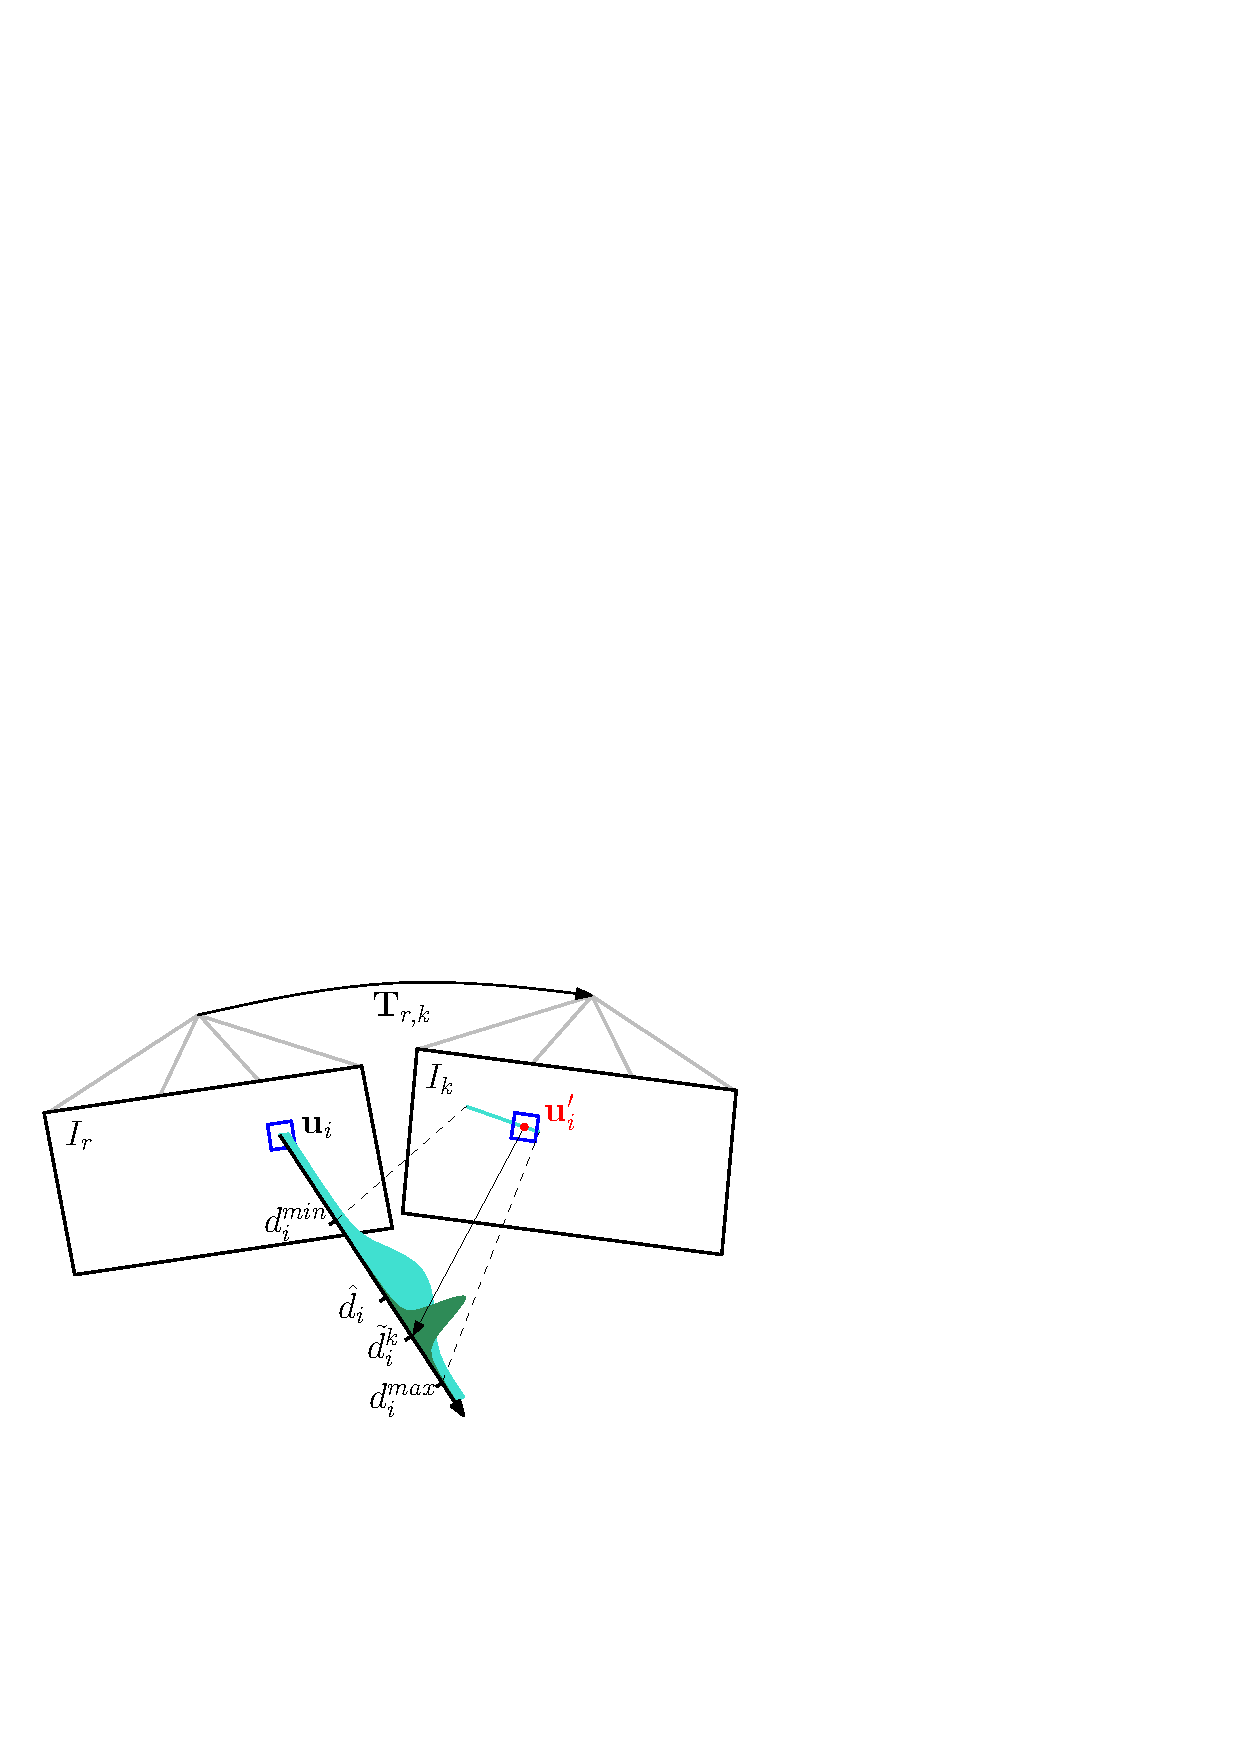
\includegraphics[width=10cm]{img/christian/vogiatzis.pdf}
  \caption{SVO depth filter \cite{Forster2014}}
  \label{fig:depth_filter}
\end{figure}

Given a point in the reference frame, its corresponding location in a new image is found by tacking a patch around the point in the reference frame, and correlating along the epipolar line in the new image. The point whose patch has maximum correlation is taken as match. Once the uncertainty of the depth distribution is low enough, its accepted in the map and used in the tracking step.\\

Featured points are only computed in keyframes and then tracked in the following frames. A new keyframe will be selected after a certain translation threshold is passed.\\

To find the pose of a new incoming frame, the following steps are performed: first, a sparse image alignment~\ref{fig:svo_img_alig} over $SE(3)$~\cite{Strasdat2012} is performed between the new frame and the last one. That is, patches from featured points whose depth is know from the last frame are projected into the new frame. The difference between patches is an error function on the transformation that is then minimized using an iterative Gauss-Newton procedure.\\

\begin{figure}[htpb]
  \centering
  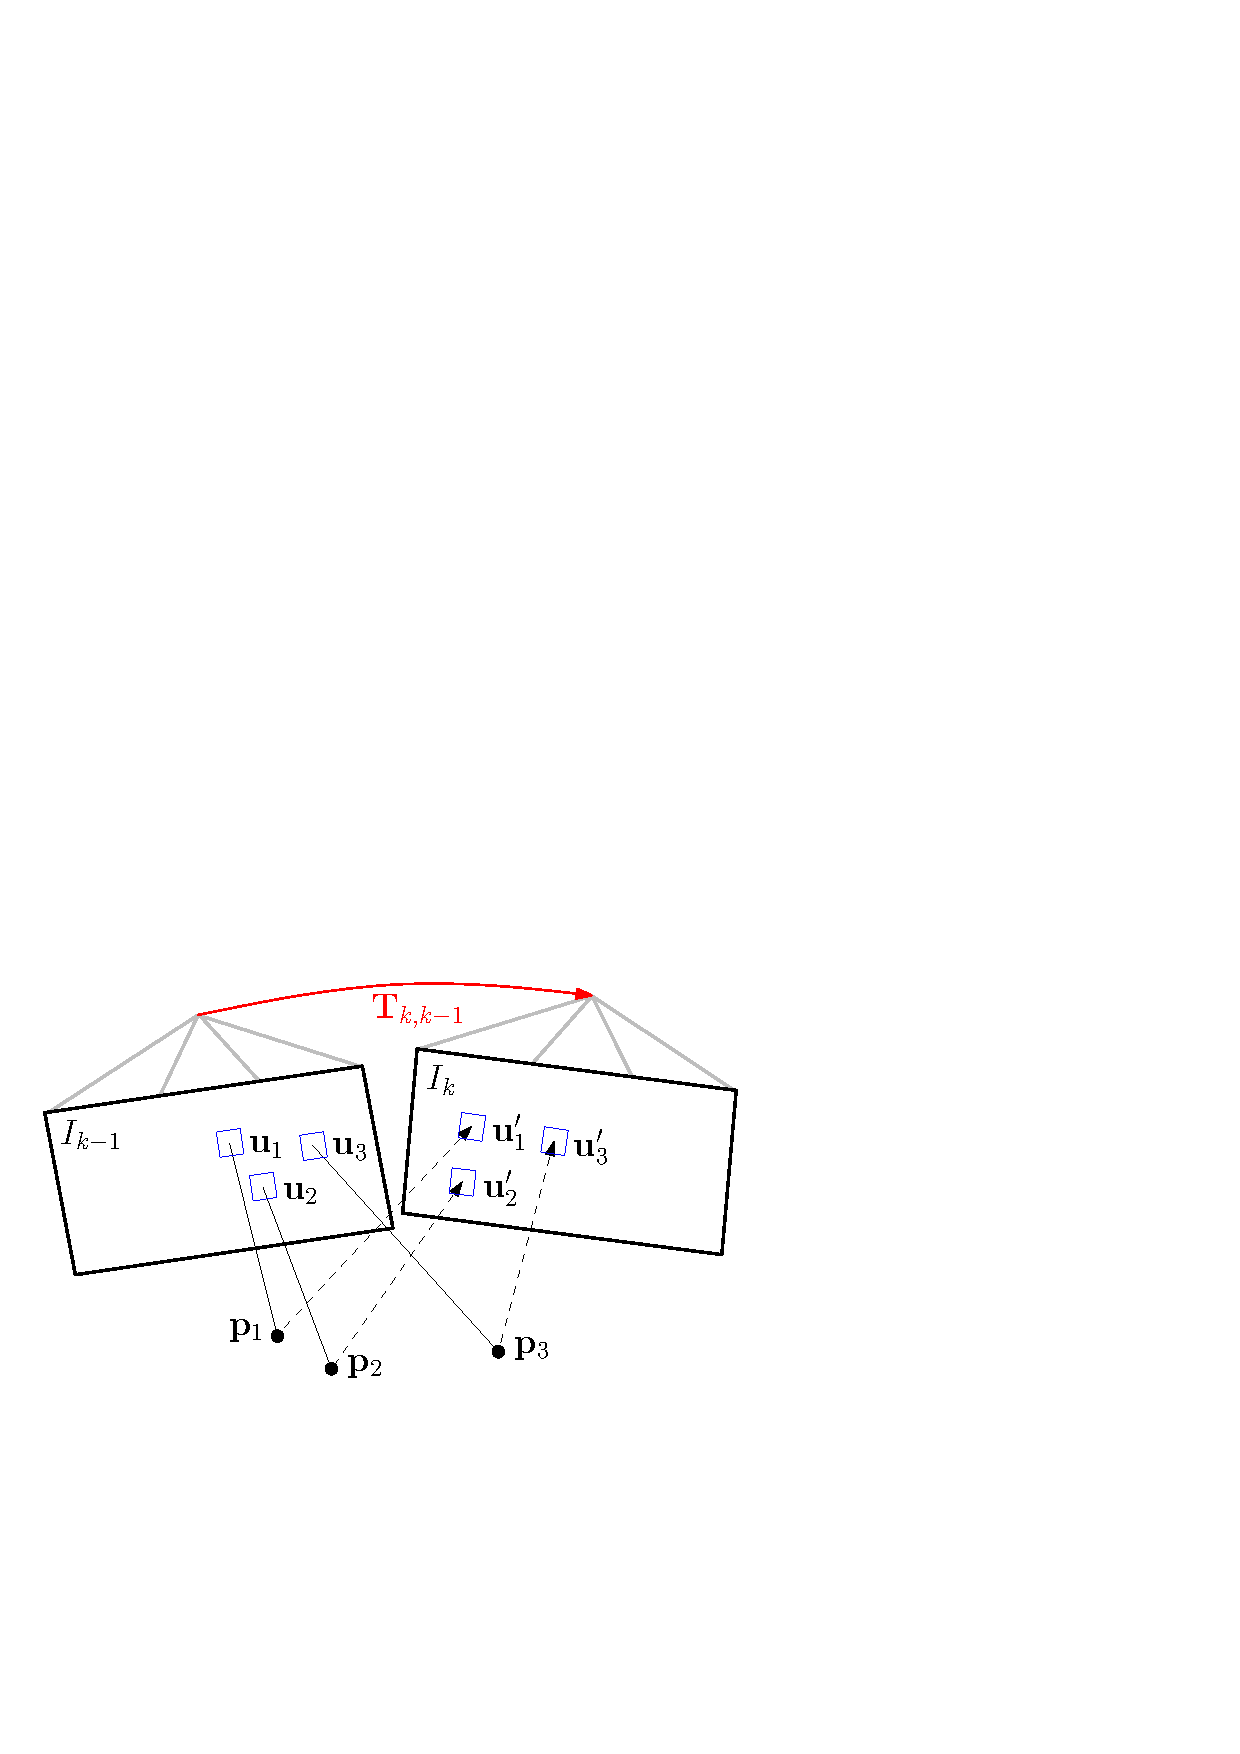
\includegraphics[width=10cm]{img/christian/sparse_img_alignment.pdf}
  \caption{SVO sparse image alignment \cite{Forster2014}}
  \label{fig:svo_img_alig}
\end{figure}

After this step a global pose of the frame is found. To improve the results not only the last frame should be used. All the points from the map, that are visible to the frame, are then projected on it straight from the keyframe where they were initially found and a similar alignment is performed as seen in~\ref{fig:svo_feature_align}. In this case, as the used frames might be farther away and the used patch is larger, an affine warp is applied to the patch. \\

\begin{figure}[htpb]
  \centering
  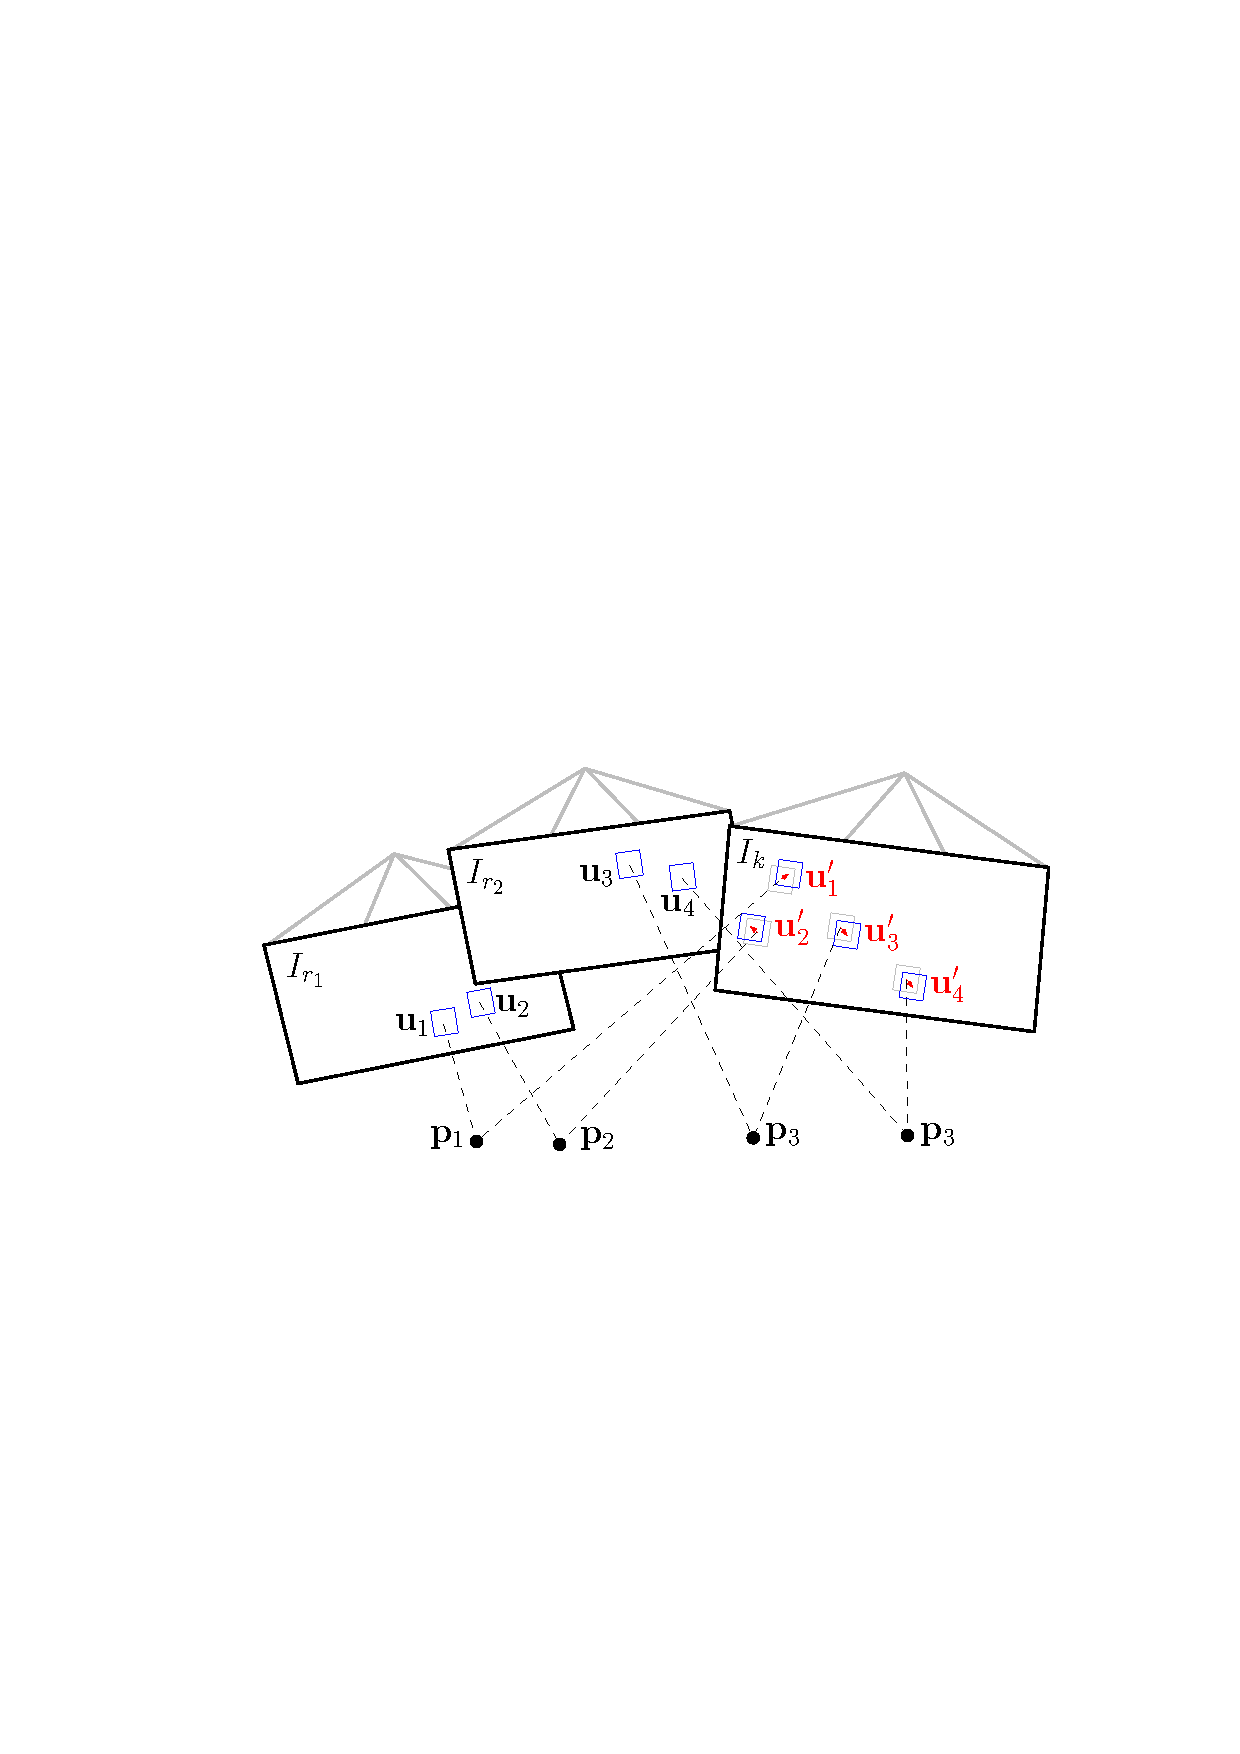
\includegraphics[width=10cm]{img/christian/feature_alignment.pdf}
  \caption{SVO feature alignment \cite{Forster2014}}
  \label{fig:svo_feature_align}
\end{figure}

Finally, Bundle Adjustment is applied to the map to optimize the pose of keyframes and the 3D location of the world points~\ref{fig:svo_global_optimization}.\\

\begin{figure}[htpb]
  \centering
  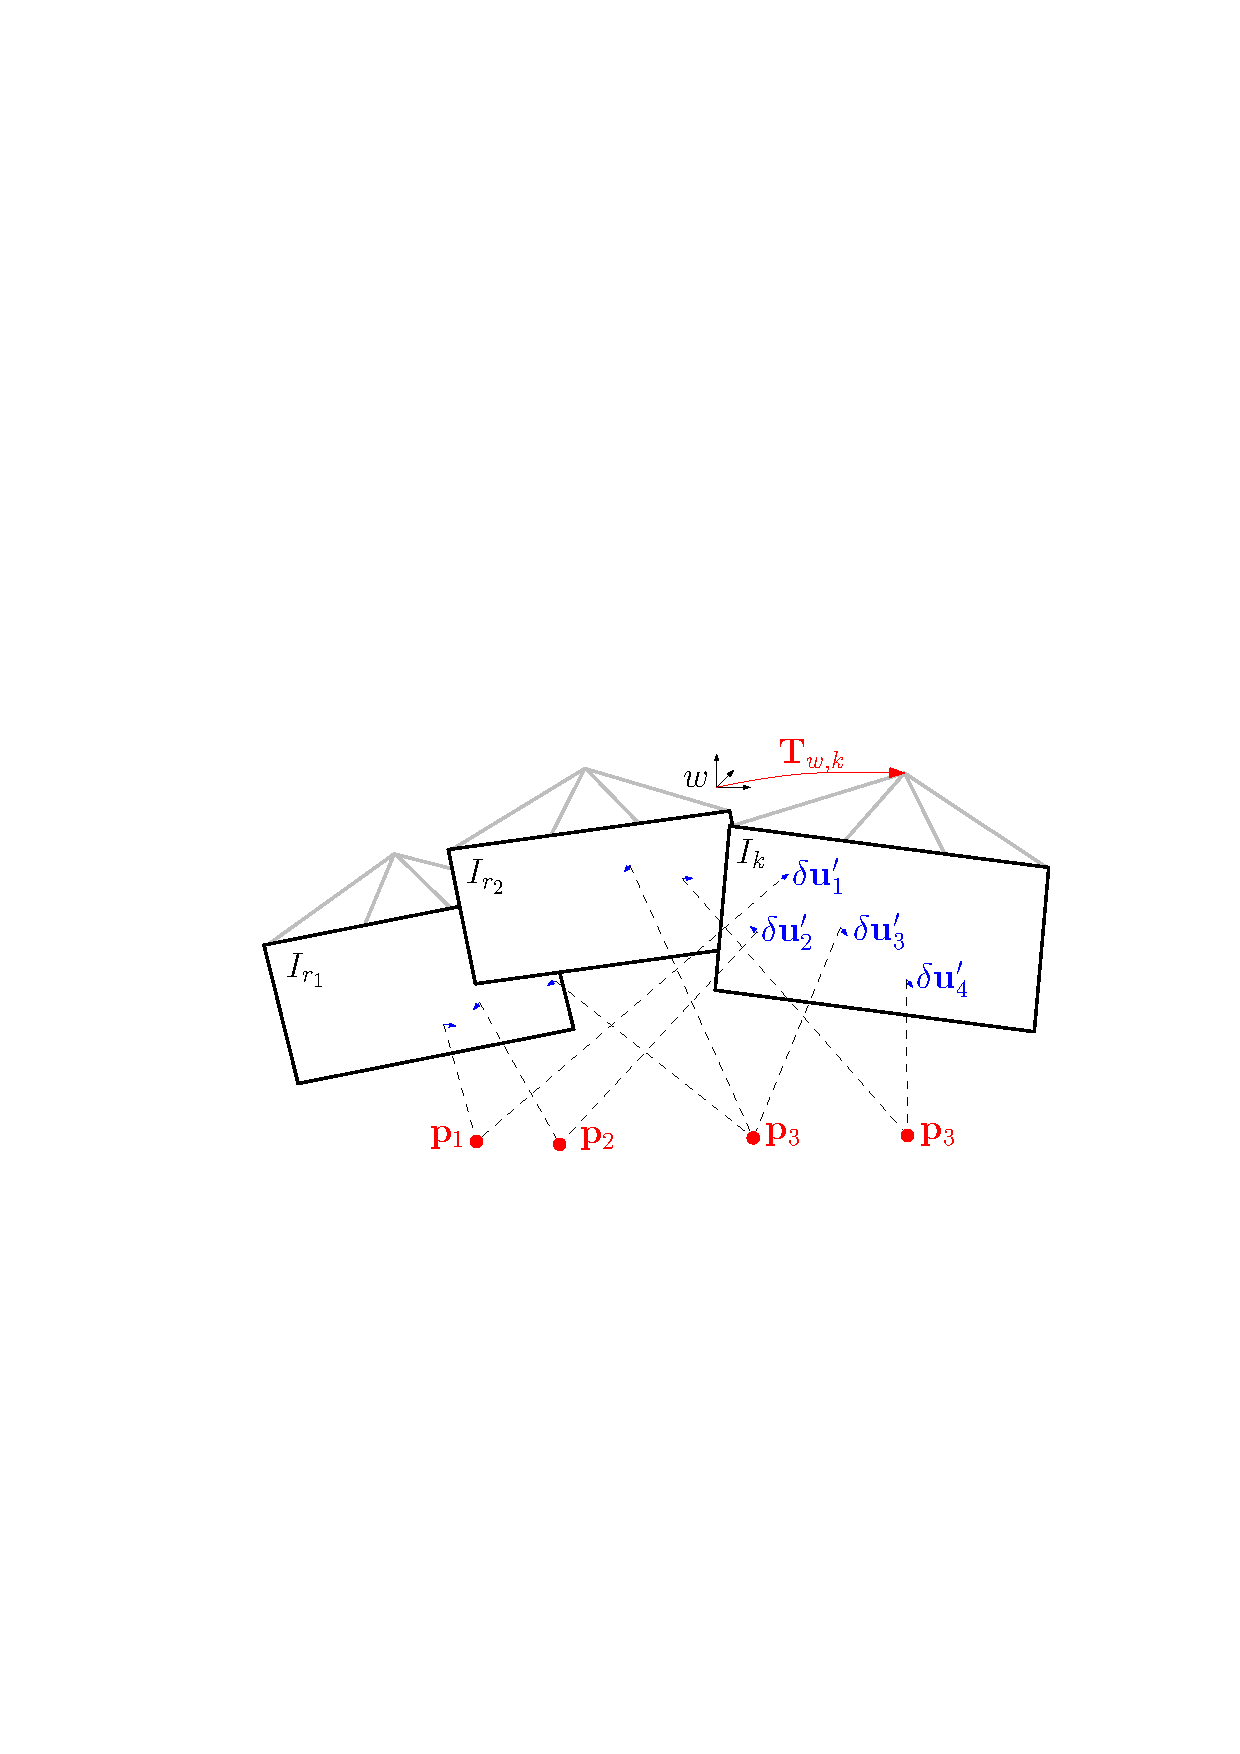
\includegraphics[width=10cm]{img/christian/pose_optimization.pdf}
  \caption{SVO global optimization \cite{Forster2014}}
  \label{fig:svo_global_optimization}
\end{figure}

\subsection{Interest point detection, descriptor extraction and matching}
\label{ssub:interest_point_detection_descriptor_extraction_and_matching}

The goal here is, given a pair of images, find points in both images that represent the same object in the world. Two things are important to achieve this. First, the point detection should be repeatable. If one point is detected in one image then it should also be detected in the second. And second, given a pair of points from two different images, there must be a way to tell if they are the same or not.\\

To achieve the repeatability, only salient points are used. These are points that, under some criterion can be distinctive from their surrounding. An early criterion for saliency was the measure of cornerness. Corners in an image are easily distinguishable. One salient point detector that uses point's cornerness is the Harris detector~\cite{harris1988combined}. Later on, many other detectors where developed, such as the Hessian or Laplacian detectors~\cite{beaudet1978rotationally}, the Difference of Gaussian detector from SIFT~\cite{lowe2004distinctive}, which tries to approximate the Laplacian.\\

Finally, to be able to tell points from different images apart, a way to compare them is needed. Intensity around to point could be used to compare, but a rotation or a change on illumination could easily, among others, make this method very unstable. To solve this problem different invariant descriptors have been developed. Descriptors are a set of $N$ values that encode the appearance of the point. This $N$ values can be regarded as a point in a $N$-dimensional space, and the distance between those can be used as a measurement of similarity.\\

The most well known descriptor and still one of the best performing one is SIFT~\cite{lowe2004distinctive}. It is a descriptor based on a histogram of gradient directions. The fact that it is based on gradient makes it invariant to illumination changes, while the fact that the histogram is sorted makes it invariant to rotation.\\

During the matching process, from two sets of descriptors, the search of the nearest neighbour of every of the values in one set is performed in the other leading to a list of pairs. This might lead to false positives like false associations and one to many associations which should be taken care of in the subsequent posterior processes. To avoid this, most image registration approaches use robust estimators~\cite{fischler1981random} that are ale to identify and reject outliers.\\





